\documentclass{article}

% Package for setting page margins
\usepackage[top=1cm, bottom=1cm, left=2cm, right=2cm]{geometry}

% Package for better font handling
\usepackage[T1]{fontenc}
\usepackage[utf8]{inputenc}
\usepackage{lmodern}
\usepackage{qrcode}
\usepackage{xcolor}
\usepackage{titlesec}
\titleformat{\section}{\large\bfseries}{\thesection}{1em}{}

% Package for customizing itemized lists
\usepackage{enumitem}
\setlist[itemize]{leftmargin=*}
 \usepackage[colorlinks=true, citecolor={red!70!black}, linkcolor={red!40!black}, urlcolor={blue!40!black}, pdfborder={0 0 0}]{hyperref}
 
% Package for including images
\usepackage{graphicx}
\usepackage{multicol}

\begin{document}


\pagestyle{empty} % Remove page numbers

% Header section with image
\begin{center}
    \begin{minipage}[t]{0.2\textwidth}
        \vspace{0pt}
        
\includegraphics[width=3cm]{img.png}
    \end{minipage}
    \hspace{1cm}
    \begin{minipage}[t]{0.7\textwidth}
        \vspace{0pt}
        \textbf{CURRICULUM VITAE}\\\\
        \textbf{Name:} Javier Alejandro Oramas López\\
        \\
        \textbf{Phone:} +53 59334374 \\
        \textbf{Email:} javiale2000@gmail.com \\
        \textbf{Date of Birth:}  02/25/2000\\
        \textbf{github:} \href{https://github.com/JavierOramas}{JavierOramas} \\
        \textbf{linkedin:} \href{https://www.linkedin.com/in/javier-alejandro-oramas-l%C3%B3pez-7ab47b160/}{javier-alejandro-oramas} \\
    \end{minipage}
\end{center}

% Education section
\section*{Education}
\textbf{Bachelors Degree Student in Computer Science} \hfill since \textbf{2018}\\
\href{https://matcom.in/}{MATCOM}, \href{https://uh.cu}{Havana University}, Cuba\\
\vspace{0.1cm}\\
\textbf{\hyperref[sec:bachelor]{Science Bachelor}} \hfill \textbf{2018}\\
Vocational Institute of Exact Sciences  Ernesto Guevara, Cuba

% % Experience section
% \section*{Experience}
% \textbf{Job Title} \hfill \textbf{Year}\\
% Company Name, Location
% \begin{itemize}
%     \item Description of responsibilities and achievements.
% \end{itemize}

% Personal Projects section
\section*{Personal Projects}
\begin{minipage}{0.8\textwidth}
\parbox{0.8\linewidth}{\textbf{Distributed file system for \href{https://autogoal.github.io/}{AutoGOAL}}}\hfill \textbf{06/2023} \\
Academic Project\\
(self discovery, failure tolerance, replication)\\
\href{https://github.com/geeksLabTech/kade-drive}{see code}\\
\end{minipage} \hfill \qrcode[height=0.6in]{https://github.com/geeksLabTech/kade-drive}\\\\
\begin{minipage}{0.8\textwidth}
\parbox{0.8\linewidth}{\textbf{Model to infer Cuba's contact matrix using Machine Learning}} \hfill \textbf{06/2023}\\
Academic Project\\
\href{https://github.com/geeksLabTech/epidemic-classification-ml-project}{see code}\\
\end{minipage} \hfill \qrcode[height=0.6in]{https://github.com/geeksLabTech/epidemic-classification-ml-project}\\\\
\begin{minipage}{0.8\textwidth}
\parbox{0.8\linewidth}{\textbf{DSL for Michaelson's language}} \hfill \textbf{01/2023}\\
Academic Project\\
Parser,lexer,syntax and semantic checkers.\\
\href{https://github.com/geeksLabTech/compilation-dsl-project}{see code}\\
\end{minipage} \hfill \qrcode[height=0.6in]{https://github.com/geeksLabTech/compilation-dsl-project}\\\\
\begin{minipage}{0.8\textwidth}
\parbox{0.8\linewidth}{\textbf{FIFA World Cup prediction using AI planification, data-driven agent-based simulation.}}  \hfill  \textbf{12/2023}\\
Academic Project\\
\href{https://github.com/geeksLabTech/FIFA_World_Cup_2022}{see code}\\
\end{minipage} \hfill \qrcode[height=0.6in]{https://github.com/geeksLabTech/FIFA_World_Cup_2022}\\\\
\begin{minipage}{0.8\textwidth}
\parbox{0.8\linewidth}{\textbf{Development of a Web Server in C for Linux}} \hfill \textbf{01/2022}\\
Academic Project\\
\href{https://github.com/geeksLabTech/web_server}{see code}\\
\end{minipage} \hfill \qrcode[height=0.6in]{https://github.com/geeksLabTech/web_server}\\\\
\begin{minipage}{0.8\textwidth}
\parbox{0.8\linewidth}{\textbf{Development of a Linux Shell in C}} \hfill \textbf{12/2021}\\
Academic Project\\
\href{https://github.com/geeksLabTech/SO_Shell}{see code}\\
\end{minipage} \hfill \qrcode[height=0.6in]{https://github.com/geeksLabTech/SO_Shell}\\\\
\begin{minipage}{0.8\textwidth}
\parbox{0.8\linewidth}{\textbf{Development of a Functional MIPS Microprocessor}} \hfill \textbf{06/2021}\\
Academic Project\\
\href{https://github.com/JavierOramas/MIPS-Micro/blob/master/informe.pdf}{see report}\\
\href{https://github.com/JavierOramas/MIPS-Micro}{see code}\\
\end{minipage} \hfill \qrcode[height=0.6in]{https://github.com/JavierOramas/MIPS-Micro}\\\\
\begin{minipage}{0.8\textwidth}
\parbox{0.8\linewidth}{\textbf{TicTacToe game using Minimax in Python}} \hfill \textbf{05/2021}\\
Academic Project\\
\href{https://github.com/JavierOramas/TicTacToe_AI}{see code}\\
\end{minipage} \hfill \qrcode[height=0.6in]{https://github.com/JavierOramas/TicTacToe_AI}\\\\
\begin{minipage}{0.8\textwidth}
\parbox{0.8\linewidth}{\textbf{Development of a Bot for FAQ automation with a knowledge base for a website}} \hfill \textbf{04/2021}\\
Academic project\\
Euclidean dot product\\
\href{https://github.com/JavierOramas/FAQ-Chat-Bot-Nous}{see code}\\
\end{minipage} \hfill \qrcode[height=0.6in]{https://github.com/JavierOramas/FAQ-Chat-Bot-Nous}\\\\
\begin{minipage}{0.8\textwidth}
\parbox{0.8\linewidth}{\textbf{Development of \hyperref[sec:laluu]{LaLuu} app for estimation of Energy consumption based on the Devices and its use time, }} \hfill \textbf{01/2021}\\
Dart/Flutter\\
\hyperref[sec:laluu_press]{Mentions about the LaLuu app in the Cuban press.}\\
\href{https://github.com/geeksLabTech/LaLuu}{see code}\\
\end{minipage} \hfill \qrcode[height=0.6in]{https://github.com/geeksLabTech/LaLuu}\\\\
\begin{minipage}{0.8\textwidth}
\parbox{0.8\linewidth}{\textbf{Development of a tool for video/audio compression}} \hfill \textbf{11/2020}\\
(video-diet, forked as diet-video for furthe development after original project being abandoned)\\
href{https://pypi.org/project/diet-video/}{pypi}\\
href{https://pypi.org/project/video-diet/}{original pypi}\\
\href{https://github.com/JavierOramas/video-diet}{see code}\\
\end{minipage} \hfill \qrcode[height=0.6in]{https://github.com/JavierOramas/video-diet}\\\\
\begin{minipage}{0.8\textwidth}
\parbox{0.8\linewidth}{\textbf{Development of a Server with web and mobile clients for microprocessor and Drives temperatures remotely.}} \hfill \textbf{08/2020}\\
Using Python fo API development, Streamlit for WebApp and Dart/Flutter for Mobile client.\\
\href{https://github.com/JavierOramas/temperatureMonitor}{see server code}\\
\href{https://github.com/JavierOramas/temperatureMonitor-app}{see app code}\\
\end{minipage} \hfill \qrcode[height=0.6in]{https://github.com/JavierOramas/temperatureMonitor}\\\\
\begin{minipage}{0.8\textwidth}
\parbox{0.8\linewidth}{\textbf{Development of \hyperref[sec:covid]{Covid19CubaData} for analysis of the COVID-19 data in Cuba}} \hfill \textbf{07/2020}\\
\href{https://github.com/covid19cuba/covid19cuba-action}{see code}\\
\end{minipage} \hfill \qrcode[height=0.6in]{https://github.com/covid19cuba/covid19cuba-action}\\\\
\begin{minipage}{0.8\textwidth}
\parbox{0.8\linewidth}{\textbf{Development of a \hyperref[sec:dengue]{Model to predict Dengue infections based on metheorological data using Machine Learning and Deep Learning}}} \hfill \textbf{02/2020}\\
\href{https://github.com/JavierOramas/DengAI}{see code}\\
\end{minipage} \hfill \qrcode[height=0.6in]{https://github.com/JavierOramas/DengAI}\\\\
\begin{minipage}{0.8\textwidth}
\parbox{0.8\linewidth}{\textbf{Development of \hyperref[sec:panamerican]{Lima 2019 Panamerican Games prediction}.}} \hfill \textbf{07/2019}\\
Academic Project\\
Using Machine Learning,  Python with SKLearn tools\\
\href{https://github.com/JavierOramas/PanamericanPredictor}{see code}\\
\end{minipage} \hfill \qrcode[height=0.6in]{https://github.com/JavierOramas/PanamericanPredictor}\\\\
\begin{minipage}{0.8\textwidth}
\parbox{0.8\linewidth}{\textbf{Development of "El Origen" videogame, using Unity with C\#.}} \hfill \textbf{02/2019}\\
Academic Project\\
\end{minipage} \\

\section*{Events}

\begin{minipage}{0.8\textwidth}
    \parbox{0.8\linewidth}{\textbf{Delegate presenting the project "Predicting Qatar 2023 World Cup, a data driven agent based approach" }} \hfill \textbf{05/2023}\\
    \hyperref[sec:workshop]{1st Artificial Intelligence and Data Science Workshop.} SaberUH Event. Math and Computation faculty. Havana University.\\
\end{minipage} \\
\begin{minipage}{0.8\textwidth}
    \parbox{0.8\linewidth}{\textbf{Forum UH, presenting Qatar 2023 predictions.}} \hfill \textbf{12/2022}\\
    Havana University.\\
\end{minipage}\\
\begin{minipage}{0.8\textwidth}
    \parbox{0.8\linewidth}{\textbf{\hyperref[sec:pythonpizza]{Python Pizza Holguín 2020}, Conference: Video-Diet: poniendo a dieta tu almacenamiento}} \hfill \textbf{11/2020}\\
\end{minipage} \\
\begin{minipage}{0.8\textwidth}
    \parbox{0.8\linewidth}{\textbf{\hyperref[sec:dengue]{Driven Data competition Predicting Dengue Cases} based on metheorological variables using Machine Learning and Deep Learning} \href{https://www.drivendata.org/competitions/44/dengai-predicting-disease-spread}{DrivenData}} \hfill \textbf{02/2020}\\
    \\
\end{minipage} \hfill \qrcode[height=0.6in]{https://www.drivendata.org/competitions/44/dengai-predicting-disease-spread}\\
\begin{minipage}{0.8\textwidth}
    \parbox{0.8\linewidth}{\textbf{\hyperref[sec:panamerican]{International contest Prediction Model for the Lima 2019 Panamerican Games results}, using Machine Learning} }\\
    \href{https://github.com/JavierOramas/PanamericanPredictor/blob/master/panamerican_predictor_paper.pdf}{see document}\\
    \href{http://www.postdata.club/issues/201907/el-medallero-de-lima-2019-que-se-puede-esperar.html}{postdata publication}\\
    \hfill \textbf{07/2019}\\
    \\
\end{minipage} \hfill \qrcode[height=0.6in]{http://www.postdata.club/issues/201907/el-medallero-de-lima-2019-que-se-puede-esperar.html}\\
\begin{minipage}{0.8\textwidth}
    \parbox{0.8\linewidth}{\textbf{MATCOM Game Festival 2019, videogame "El Origen" (The Origin)
    }} \hfill \textbf{02/2019}\\
    \\
\end{minipage}\\
\begin{minipage}{0.8\textwidth}
    \parbox{0.8\linewidth}{\textbf{ACM-ICPC 2018 National Contest, UH-KEJ (Participating as a team representing Havana University)} }\hfill \textbf{10/2018}\\
    \href{https://icpc.global/regionals/finder/cnc-2018/standings}{standings}
    \\
\end{minipage} \hfill \qrcode[height=0.6in]{https://icpc.global/regionals/finder/cnc-2018/standings}\\
\begin{minipage}{0.8\textwidth}
    \parbox{0.8\linewidth}{\textbf{ACM-ICPC 2018 Local Contest, UH-KEJ  (Participating as a team representing Havana University)}} \hfill \textbf{07/2018}\\
    \\
\end{minipage} \hfill \qrcode[height=0.6in]{https://matcomgrader.com/post/5179/resultados-del-concurso-local-caribeno-2018}\\
\begin{minipage}{0.8\textwidth}
    \parbox{0.8\linewidth}{\textbf{ACM-ICPC 2017 Caribbean Final, Team3C-1 (Participating as  Invited Team from pre-universitary schools)
    Invitation Letter from the General Director, Caribbean Final ACM - ICPC 2017}} \hfill \textbf{11/2017}\\
    \href{https://matcomgrader.com/post/5167/the-2017-acm-icpc-caribbean-finals}{see link}
    \href{https://coj-forum.uci.cu/viewtopic.php?t=3315}{coj (competition) page}
    \\
\end{minipage} \hfill \qrcode[height=0.6in]{https://matcomgrader.com/post/5167/the-2017-acm-icpc-caribbean-finals}\\
\begin{minipage}{0.8\textwidth}
    \parbox{0.8\linewidth}{\textbf{ACM-ICPC 2017 Cuban Final, Team3C-1 (Participating as  Invited Team from pre-universitary schools)}} \hfill \textbf{10/2017}\\
    \\
\end{minipage}\\
\begin{minipage}{0.8\textwidth}
    \parbox{0.8\linewidth}{\textbf{Cuban Olimpiad in Informatics 2016-2017, for pre-universitary students in Cuba.}} \hfill \textbf{03/2017}\\
    \\
\end{minipage}\\
\begin{minipage}{0.8\textwidth}
    \parbox{0.8\linewidth}{\textbf{\hyperref[sec:ibero]{Ibero-american Computer Correspondence Contest} , México 2016, representing  Cuba.}} \hfill \textbf{07/2016}\\
    \\
\end{minipage}\\
\begin{minipage}{0.8\textwidth}
    \parbox{0.8\linewidth}{\textbf{National pre-selection for International Olimpiad in Informatics.}} \hfill \textbf{04-07/2016}\\
    \\
\end{minipage}\\
\begin{minipage}{0.8\textwidth}
    \parbox{0.8\linewidth}{\textbf{Lenin Cup, Computer Contest for pre-universitary Students in Cuba.}} \hfill \textbf{01/2016}\\
    \\
\end{minipage}\\
\begin{minipage}{0.8\textwidth}
    \parbox{0.8\linewidth}{\textbf{Copa Regional de Concurso de Inform?tica, Camag?ey 2015 for pre-universitary students in Cuba}} \hfill \textbf{12/2015}\\
    \\
\end{minipage}\\
\begin{minipage}{0.8\textwidth}
    \parbox{0.8\linewidth}{\textbf{ACM-ICPC National Contest 2015-2016, Team3C-1 (Participating as  Invited Team from pre-universitary schools)}} \hfill \textbf{10/2015}\\
    \\
\end{minipage}\\
\begin{minipage}{0.8\textwidth}
    \parbox{0.8\linewidth}{\textbf{ACM-ICPC Local Contest 2015-2016, Team3C-1 (Participating as  Invited Team from pre-universitary schools)}} \hfill \textbf{09/2015}\\
    \\
\end{minipage}\\
\begin{minipage}{0.8\textwidth}
    \parbox{0.8\linewidth}{\textbf{Cuban Olimpiad in Informatics 2013-2014, for pre-universitary students in Cuba.}} \hfill \textbf{02/2014}\\
    \\
\end{minipage}\\
\section*{Awards and Distinctions}
\begin{minipage}{0.8\textwidth}
    \parbox{0.8\linewidth}{\textbf{Best Prediction in the world at FIFA World Cup}} \hfill \textbf{12/2022}\\
    \href{https://www.postdata.club/suplementos/mundial-qatar/pronosticando-qatar.html}{postdata.club}
    \\
\end{minipage} \hfill \qrcode[height=0.6in]{https://www.postdata.club/suplementos/mundial-qatar/pronosticando-qatar.html}\\
\begin{minipage}{0.8\textwidth}
    \parbox{0.8\linewidth}{\textbf{Best preditction int the world (for cuban delegation results) at Lima 2019 Panamerican Games, using Machine Learning}} \hfill \textbf{07/2019}\\
    \href{http://www.postdata.club/issues/201907/el-medallero-de-lima-2019-que-se-puede-esperar.html}{postdata.club}
    \\
\end{minipage} \hfill \qrcode[height=0.6in]{https://github.com/JavierOramas/PanamericanPredictor}\\
\begin{minipage}{0.8\textwidth}
    \parbox{0.8\linewidth}{\textbf{3rd place MATCOM Game Festival 2019, Videogame "El Origen"}} \hfill \textbf{02/2019}\\
    \\
\end{minipage}\\
\begin{minipage}{0.8\textwidth}
    \parbox{0.8\linewidth}{\textbf{13th place in the Caribbean, ACM-ICPC 2018 national Contest,  UH-KEJ (Participating as a team representing Havana University)}} \hfill \textbf{10/2018}\\
    \href{https://icpc.global/regionals/finder/cnc-2018/standings}{standings}
    \\
\end{minipage} \hfill \qrcode[height=0.6in]{https://icpc.global/regionals/finder/cnc-2018/standings}\\
\begin{minipage}{0.8\textwidth}
    \parbox{0.8\linewidth}{\textbf{7th place ACM-ICPC 2018 Local Contest, UH-KEJ (Participating as a team representing Havana University)}} \hfill \textbf{07/2018}\\
    \href{https://matcomgrader.com/post/5179/resultados-del-concurso-local-caribeno-2018}{standings}
    \\
\end{minipage} \hfill \qrcode[height=0.6in]{https://matcomgrader.com/post/5179/resultados-del-concurso-local-caribeno-2018}\\
\begin{minipage}{0.8\textwidth}
    \parbox{0.8\linewidth}{\textbf{Granted directly, by resolution of the Ministry of Education the career: Computer Science at Universidad de La Habana, According to the achievents in  the ACM-ICPC 2017 Caribbean Finals.}} \hfill \textbf{06/2018}\\
    \\
\end{minipage} \\
\begin{minipage}{0.8\textwidth}
    \parbox{0.8\linewidth}{\textbf{26th place in the Caribbean y 200th in LATAM, ACM-ICPC Caribbean Finals, Team3C-1 (Participating as  Invited Team from pre-universitary schools)}} \hfill \textbf{11/2017}\\
    \href{https://matcomgrader.com/media/posts/5167/ranking/caribbean.png}{Region Standing}
    \href{https://matcomgrader.com/media/posts/5167/ranking/general.png}{Continent Standing}
    \\
\end{minipage} \hfill \qrcode[height=0.6in]{https://matcomgrader.com/media/posts/5167/ranking/caribbean.png}\\
\begin{minipage}{0.8\textwidth}
    \parbox{0.8\linewidth}{\textbf{5th Place in Cuban Finals of ACM-ICPC, Team3C-1}} \hfill \textbf{10/2017}\\
    \\
\end{minipage}\\
\begin{minipage}{0.8\textwidth}
    \parbox{0.8\linewidth}{\textbf{Third Place in "UCLV CUP" proggramming contest at Universidad Central Marta Abreu de Las Villas}} \hfill \textbf{06/2017}\\
    \\
\end{minipage}\\
\begin{minipage}{0.8\textwidth}
    \parbox{0.8\linewidth}{\textbf{1st place Cuban National Programming Contest}} \hfill \textbf{01/2017}\\
    \\
\end{minipage}\\
\begin{minipage}{0.8\textwidth}
    \parbox{0.8\linewidth}{\textbf{4th place Lenin Cup}} \hfill \textbf{01/2017}\\
    \\
\end{minipage}\\
\begin{minipage}{0.8\textwidth}
    \parbox{0.8\linewidth}{\textbf{1st place at UCLV site ACM-ICPC National Finals 2015-2016 }} \hfill \textbf{10/2015}\\
    \\
\end{minipage} \\
\begin{minipage}{0.8\textwidth}
    \parbox{0.8\linewidth}{\textbf{3rd  place at UCLV site ACM-ICPC Local Finals 2015-2016 (Participating as  Invited Team from pre-universitary schools)}} \hfill \textbf{09/2015}\\
    \\
\end{minipage}\\

\section*{Membersips}

\begin{minipage}{0.8\textwidth}
    \parbox{0.8\linewidth}{\textbf{Research Group in Artifitial Intelligence at Facultad de Matemática y Computación de la Universidad de La Habana (Computer Science and Mathematics Faculty, Havana University)
    }} \hfill \textbf{Since 2019}\\
    \\
\end{minipage}\\
\begin{minipage}{0.8\textwidth}
    \parbox{0.8\linewidth}{\textbf{Cuban National pre-selection to the Intenational Olimpiad in Informatics
    }} \hfill \textbf{04/2016-07/2016}\\
    \\
\end{minipage}\\
\begin{minipage}{0.8\textwidth}
    \parbox{0.8\linewidth}{\textbf{Provincial Contest Center, Villa Clara, Cuba
    }} \hfill \textbf{04/2016-07/2016}\\
    \\
\end{minipage}\\

\newpage
% Skills section
\section*{Skills}
% \begin{minipage}{0.8\textwidth}
\begin{multicols}{2}
\raggedcolumns
\textbf{Programming Languages}
\begin{itemize}
    \item Python
    \item C
    \item C++
    \item C\#
    \item SQL
    \item Rust
    \item Go
    \item Dart
    \item Haskell
    \item Javascript
\end{itemize}
\columnbreak
\textbf{Other Technologies}
\begin{itemize}
    \item SKLearn
    \item Transformers
    \item Tensorflow
    \item Pytorch
    \item Git/Github
    \item LaTeX
    \item HTML/CSS
    \item Flutter
    \item Jupyter Notebook
    \item Fastapi
    \item Typer
    \item Beautiful soup
    \item Streamlit
    \item Pandas
    \item Numpy
\end{itemize}
\end{multicols}
% \end{minipage}\\


\newpage
\section*{Attachments}
% \begin{minipage}{0.8\textwidth}
\begin{figure}[h]
    
\includegraphics[width=\textwidth]{images/bachelor.png}
    \caption{Science Bachelor certificate}
    \label{sec:bachelor}
\end{figure}

\begin{figure}[h]
    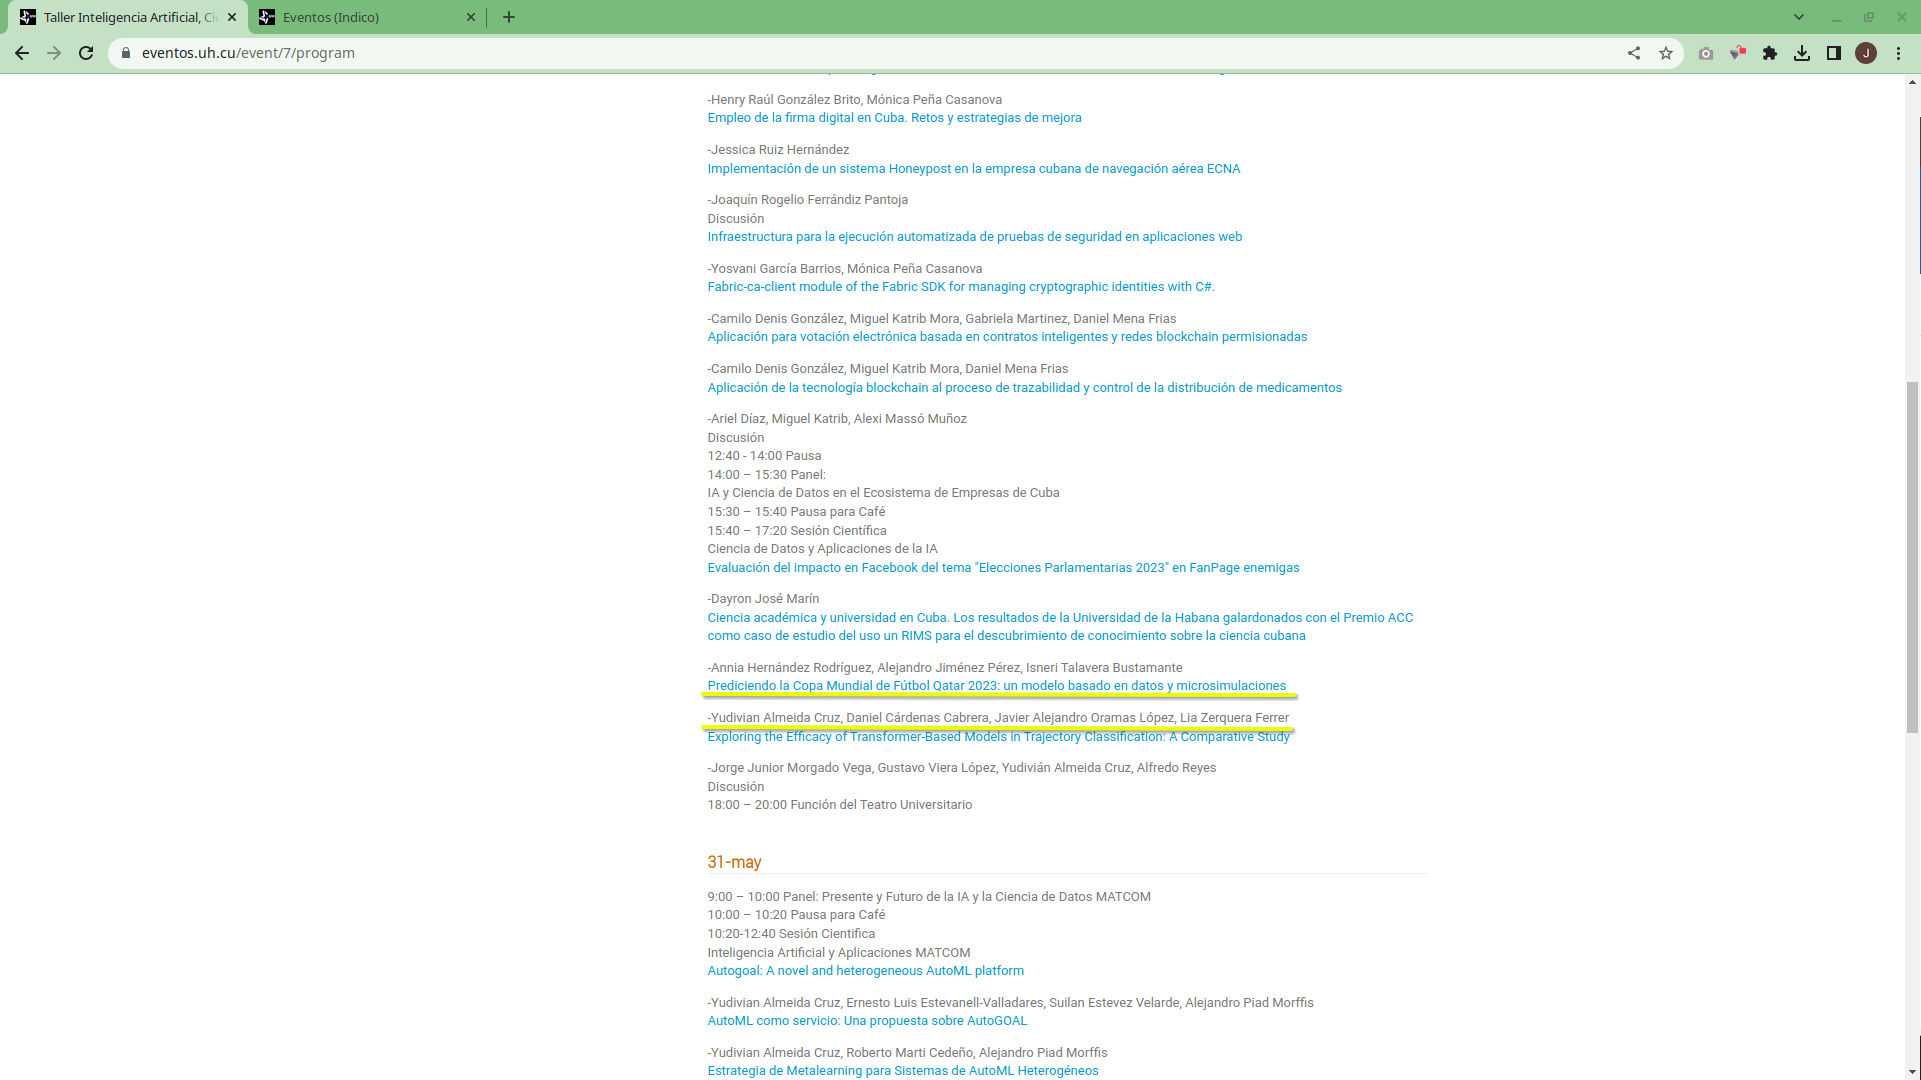
\includegraphics[width=\textwidth]{images/ai_workshop.png}
    \caption{\href{https://eventos.uh.cu/event/7/program}{Havana University events webpage}, screenshot 06/01/2023}
    \label{sec:workshop}
\end{figure}

\begin{figure}[h]
    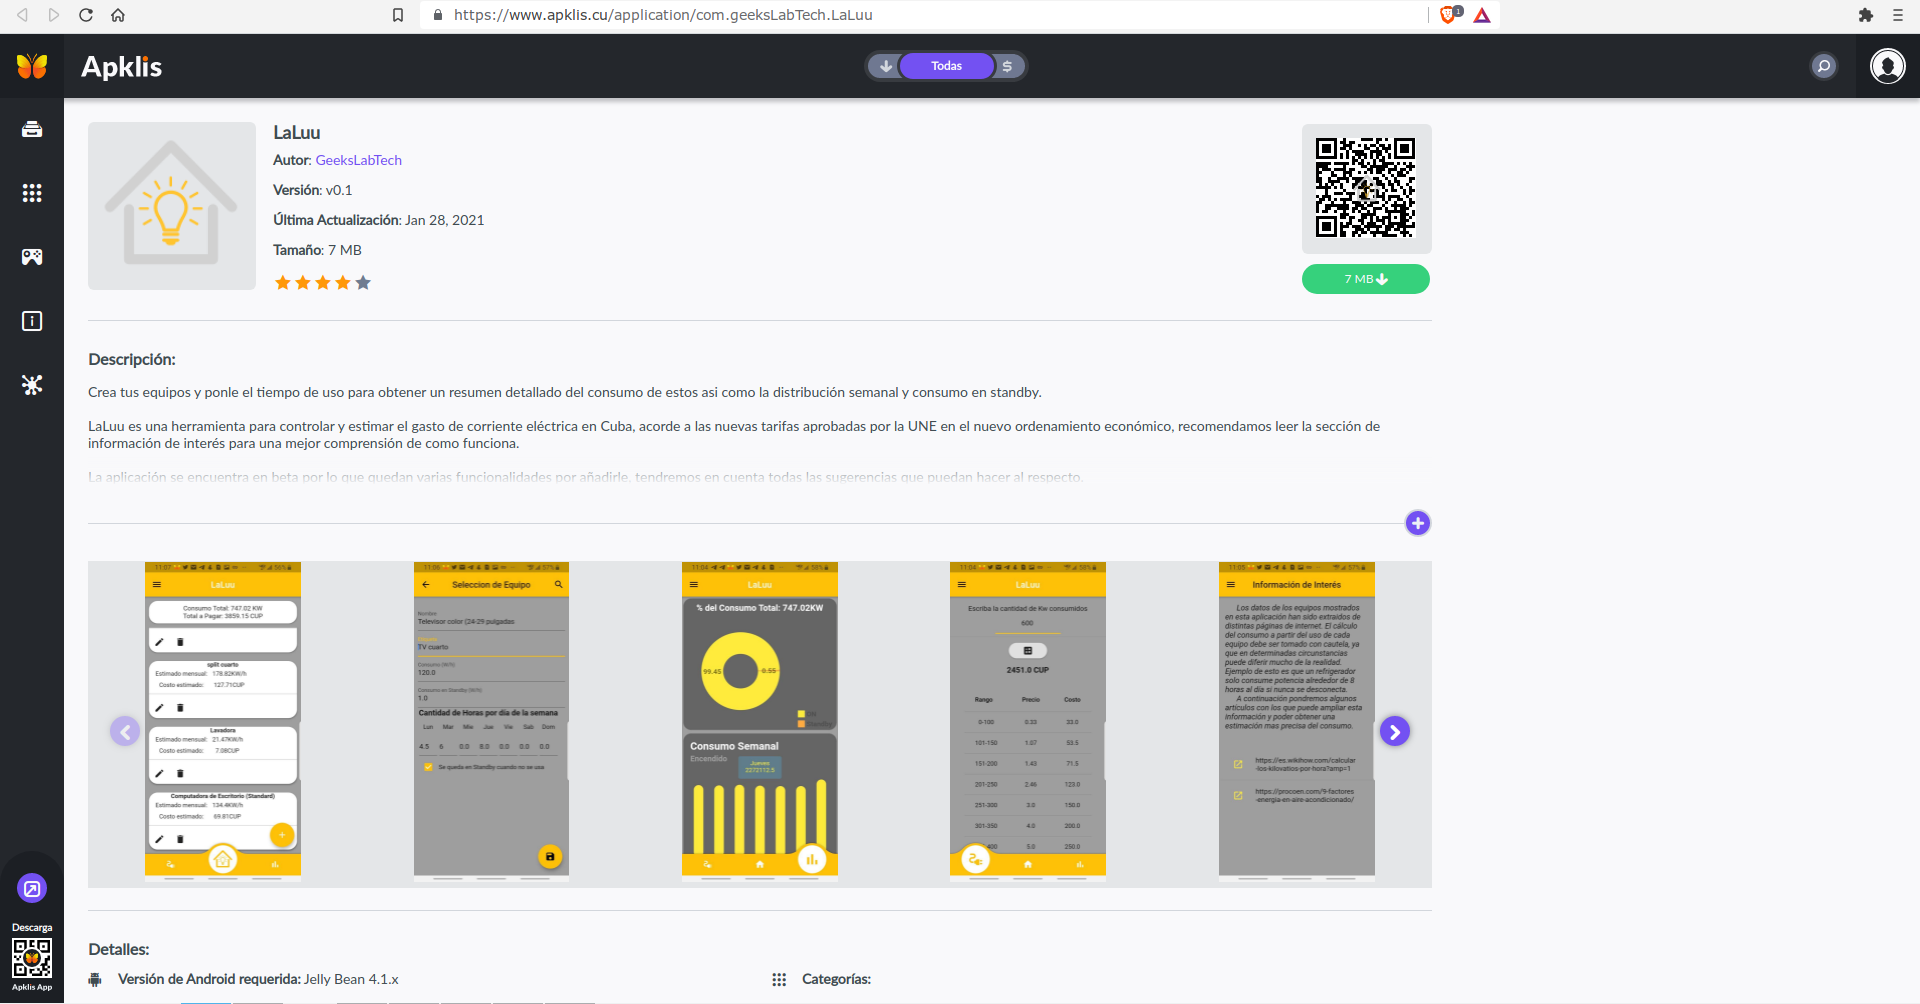
\includegraphics[width=\textwidth]{images/laluu.png}
    \caption{LaLuu app for estimation of Energy consumption. Available in \href{https://www.apklis.cu/application/com.geeksLabTech.LaLuu}{Apklis}, Cuban android app store, screenshot 01/25/2022}
    \label{sec:laluu}
\end{figure}

\begin{figure}[h]
    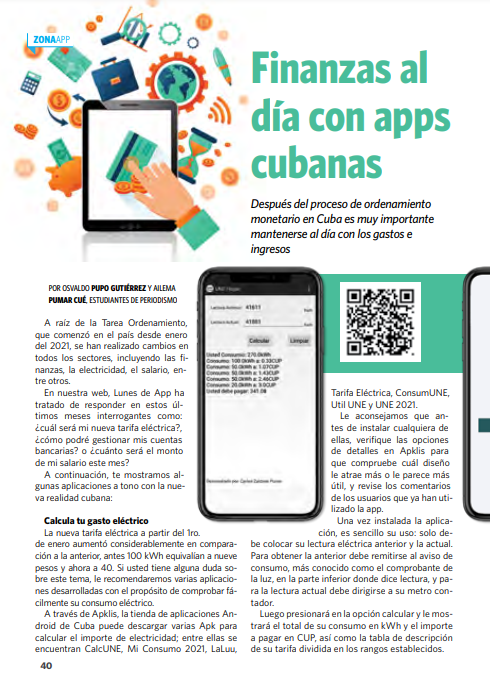
\includegraphics[width=\textwidth]{images/laluu_jt.png}
    \caption{Pupo, Gutiérrez O. y Pumar, Cué A. (may-jun 2021). \href{http://www.juventudtecnica.cu/sites/default/files/jt_420.pdf}{Finanzas al día con apps cubanas}. Juventud Técnica 420 (40-41), ISSN: 0449-4555, screenshot 01/25/2022}
    \label{sec:laluu_press}
\end{figure}

\begin{figure}[h]
    
\includegraphics[width=\textwidth]{images/laluu_art.png}
    \caption{Red Artemisa (february 2nd 2021).\href{https://www.artemisa.gob.cu/es/actualidad/noticias/9806-llego-febrero-calcula-tu-gasto-electrico-con-esta-apps}{Llegó febrero: calcula tu gasto eléctrico con esta apps.}, screenshot 01/25/2022}
\end{figure}

\begin{figure}[h]
    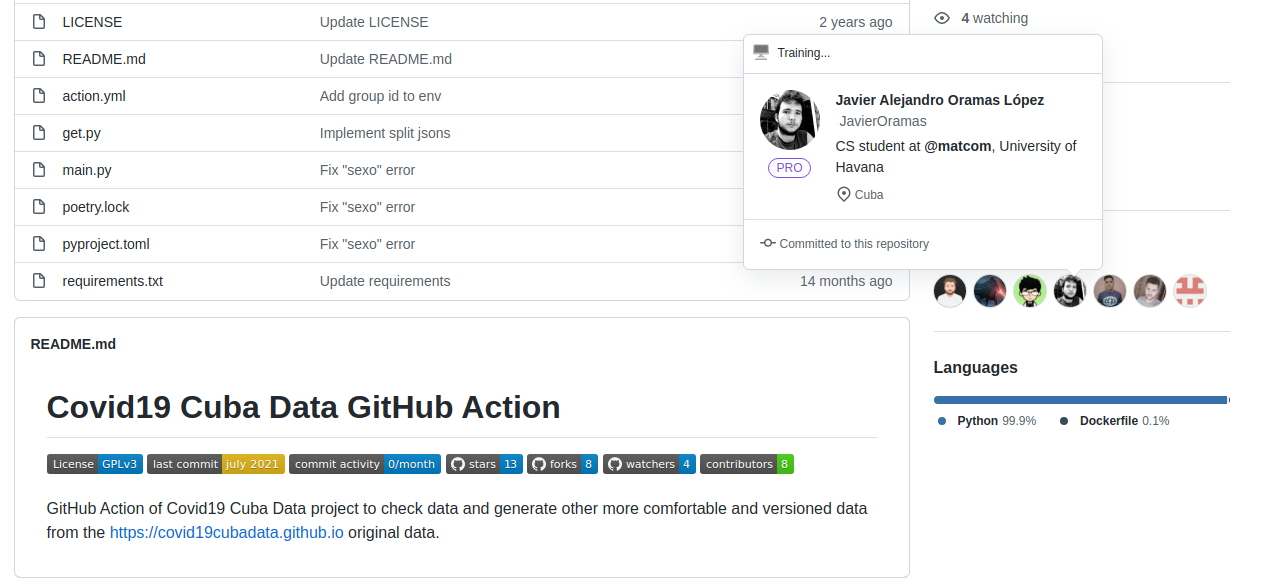
\includegraphics[width=\textwidth]{images/covid_19.png}
    \caption{\href{https://github.com/covid19cuba/covid19cuba-action}{Covid19CubaData app COVID-19 data analisys in Cuba}, screenshot 01/25/2022}
    \label{sec:covid}
\end{figure}

\begin{figure}[h]
    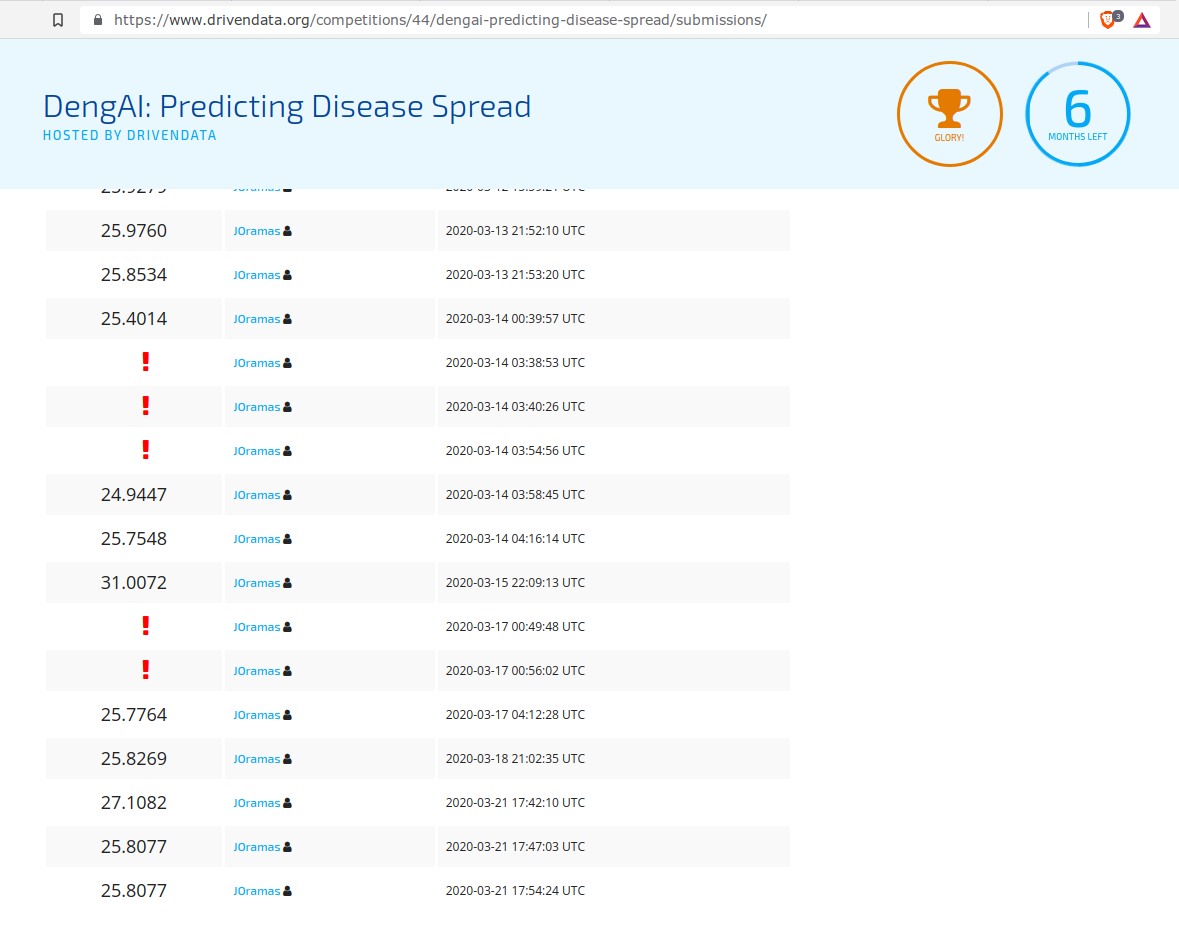
\includegraphics[width=\textwidth]{images/dengue.png}
    \caption{Competition Predicting Dengue Cases based on metheorological variables, using Machine Learning and Deep Learning. \href{https://www.drivendata.org/competitions/44/dengai-predicting-disease-spread}{DrivenData}, screenshot 01/25/2022}
    \label{sec:dengue}
\end{figure}

\begin{figure}[h]
    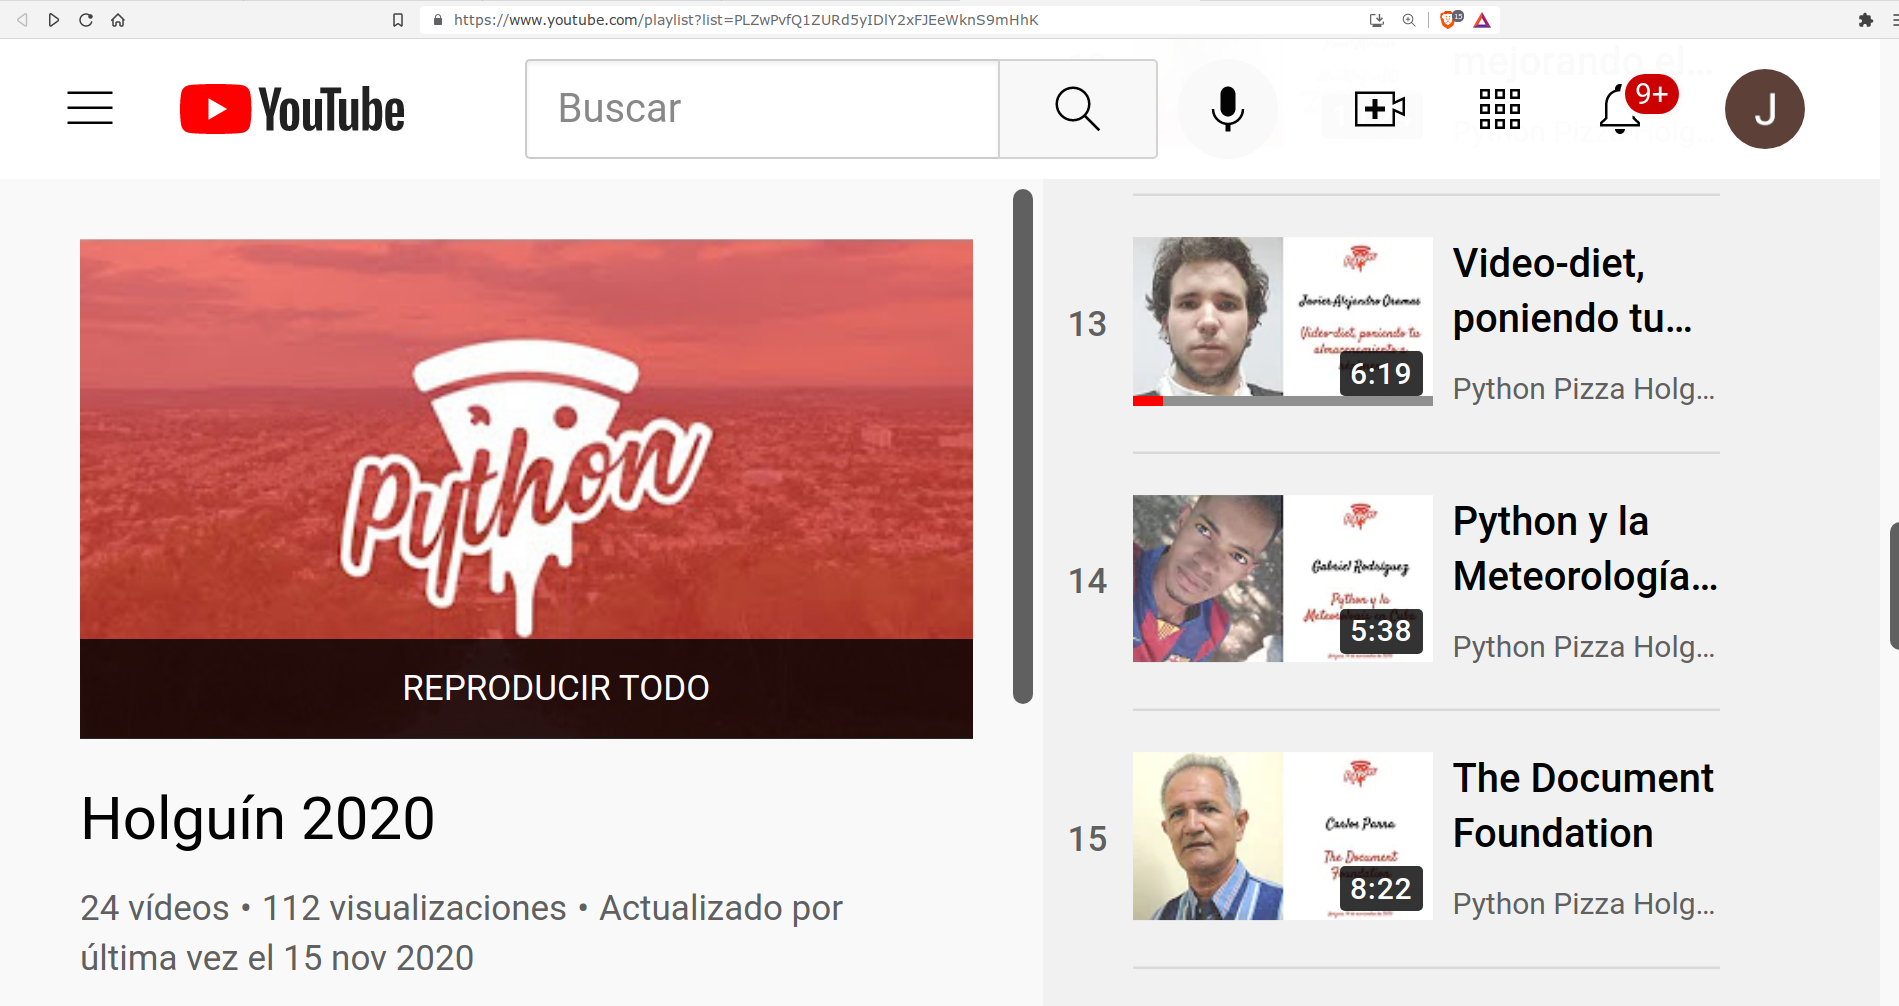
\includegraphics[width=\textwidth]{images/pythonpizza.png}
    \caption{Oramas, J. \href{https://holguin.python.pizza/?ref=python.pizza}{[Python Pizza Holguín]}. (nov 15th 2020). Video-Diet: poniendo a dieta tu almacenamiento \href{https://youtu.be/c--NOwM5W-0}{[Video]}.screenshot 01/25/2022}
    \label{sec:pythonpizza}
\end{figure}

\begin{figure}[h]
    \centering
    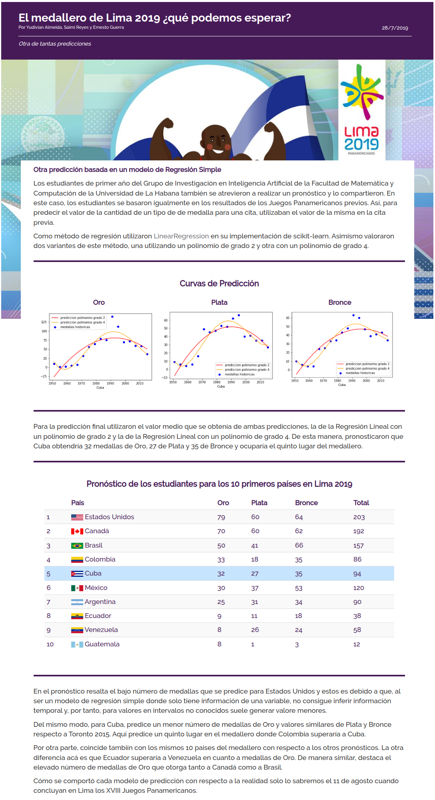
\includegraphics[height=0.8\textheight]{images/panamerican.png}
    \caption{\href{http://www.postdata.club/issues/201907/el-medallero-de-lima-2019-que-se-puede-esperar.html}{Almeida, Y. , Reyes, S. y Guerra, E. (jul 28th 2019). El medallero de Lima 2019 ¿qué podemos esperar? PostData.club Periodismo de Datos.}, screenshot 01/25/2022}
    \label{sec:panamerican}
\end{figure}

\begin{figure}[h]
    \centering
    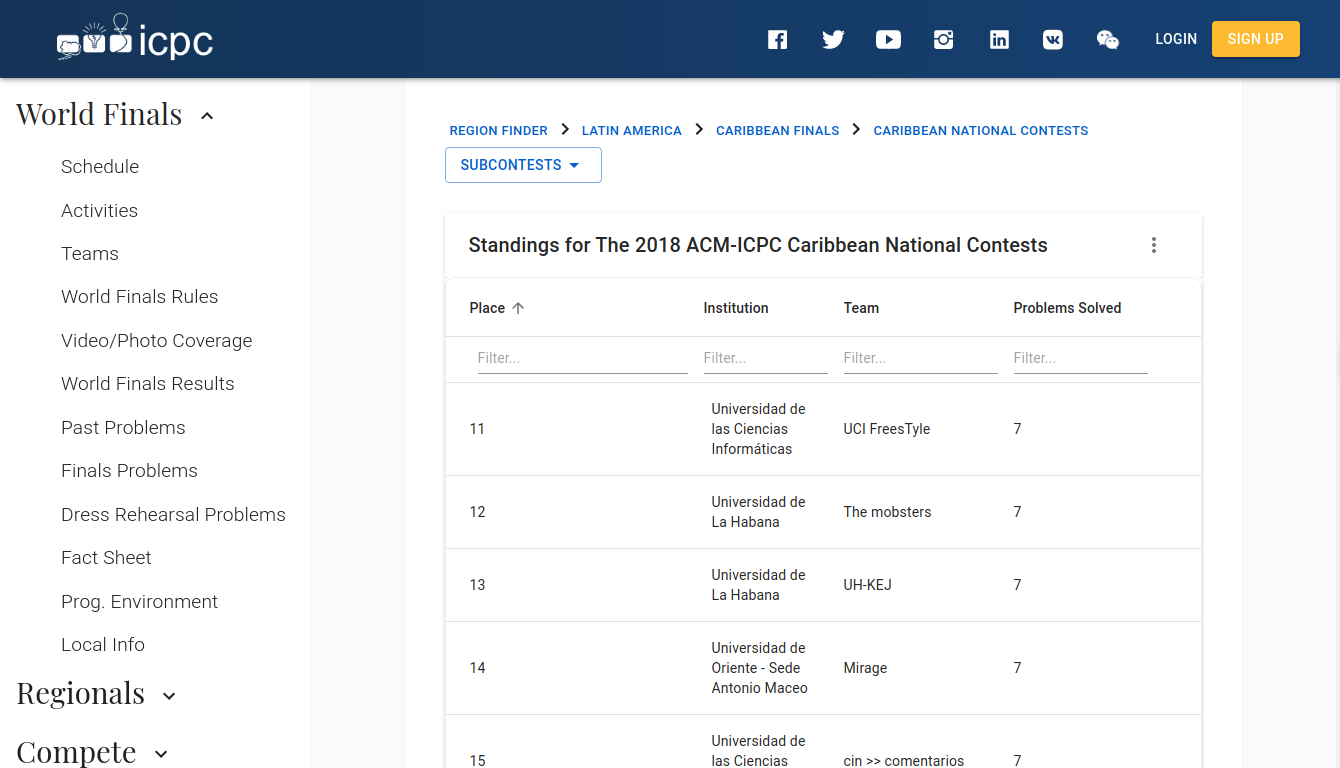
\includegraphics[width=\textwidth]{images/icpckej.png}
    \caption{ \href{https://icpc.global/regionals/finder/cnc-2018/standings}{International Collegiate Programming Contest (oct 2018). Standings for The 2018 ACM-ICPC Caribbean National Contests}. screenshot 01/25/2022}
    \label{sec:icpc_kej}
\end{figure}

\begin{figure}[h]
    \centering
    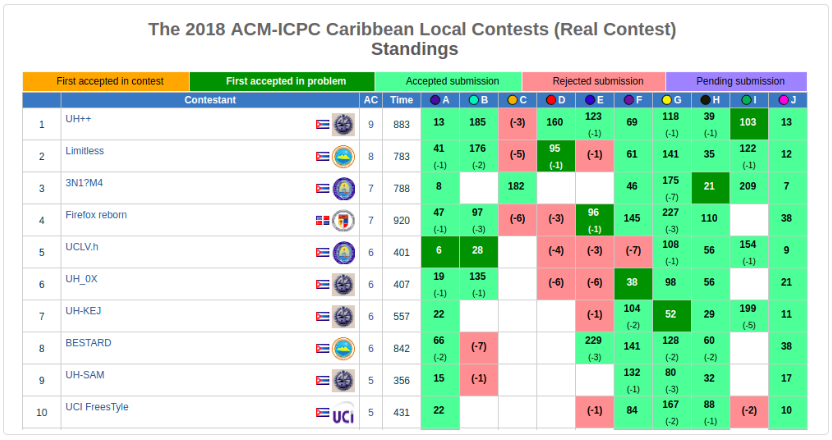
\includegraphics[width=\textwidth]{images/icpckej_standing.png}
    \caption{\href{https://matcomgrader.com/post/5179/resultados-del-concurso-local-caribeno-2018}{Matcom Online Grader (sept 2018). Resultados del Concurso Local Caribeño 2018. Facultad de Matemática y Ciencia de la Computación, Universidad de La Habana.}, screenshot 01/25/2022}
    % \label{sec:}
\end{figure}

\begin{figure}[h]
    \centering
    
\includegraphics[width=\textwidth]{images/letter.png}
    \caption{General Director invitation letter, Caribbean Finals ACM - ICPC 2017, screenshot 01/25/2022}
    \label{sec:letter}
\end{figure}

\begin{figure}[h]
    \centering
    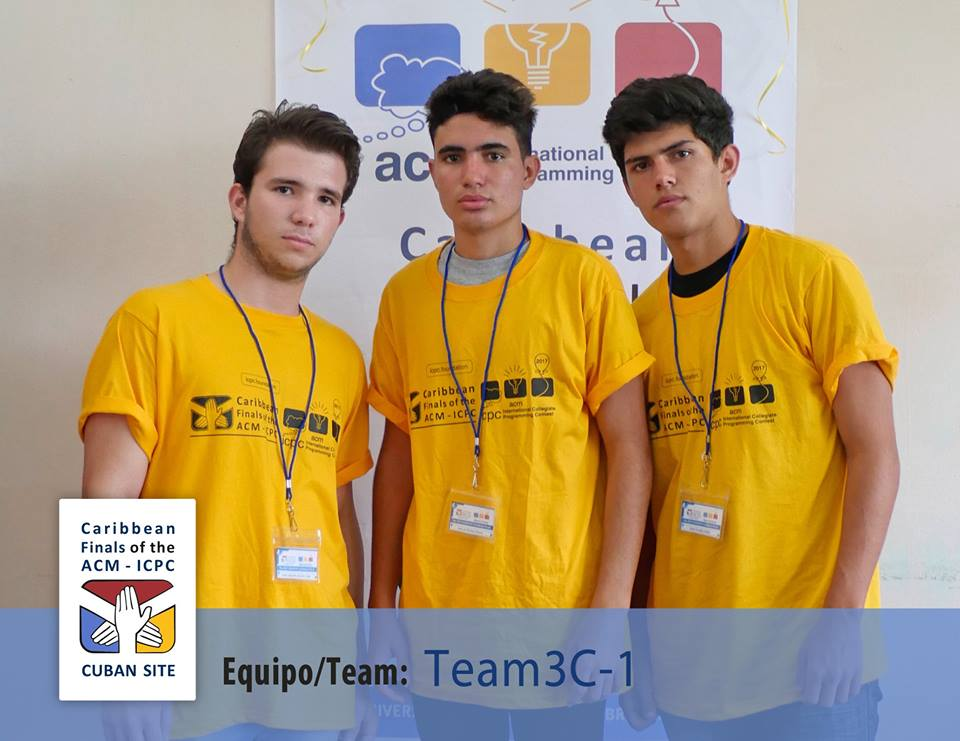
\includegraphics[width=\textwidth]{images/team3c.jpg}
    \caption{\href{https://matcomgrader.com/post/5167/the-2017-acm-icpc-caribbean-finals}{Matcom Online Grader (oct 2017). The 2017 ACM-ICPC Caribbean Finals. Facultad de Matem?tica y Ciencia de la Computaci?n, Universidad de La Habana} screenshot 01/25/2022}
    \label{sec:3c}
\end{figure}
\begin{figure}[h]
    \centering
    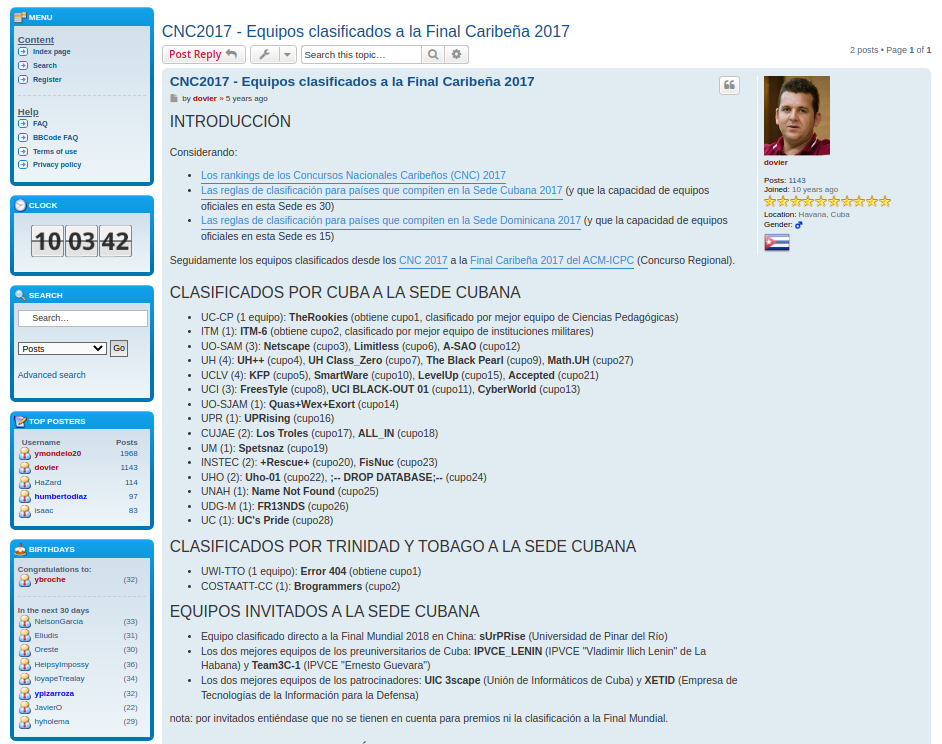
\includegraphics[width=\textwidth]{images/icpc_classified.png}
    \caption{\href{ https://coj-forum.uci.cu/viewtopic.php?t=3315}{Caribbean Online Judge (nov 2017). Final Caribe?a del ACM - ICPC 2017.}, screenshot 01/25/2022}
    \label{sec:icpc}
\end{figure}

\begin{figure}[h]
    \centering
    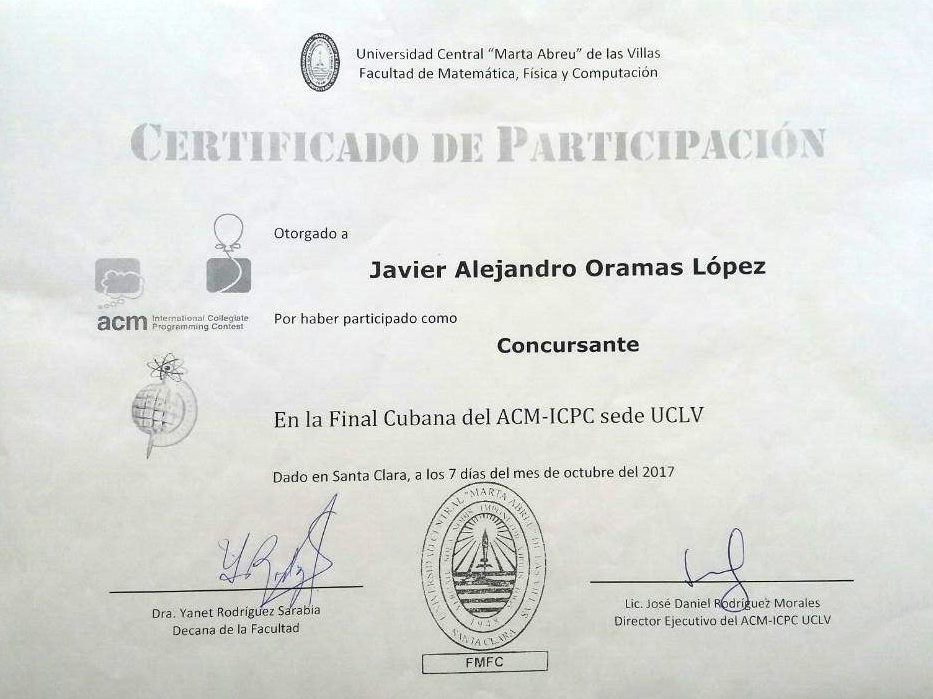
\includegraphics[width=\textwidth]{images/2017final.png}
    \caption{Participation Certificate, ACM-ICPC 2017 Cuban Finals, screenshot 01/25/2022}
    \label{sec:2017final}
\end{figure}


\begin{figure}[h]
    \centering
    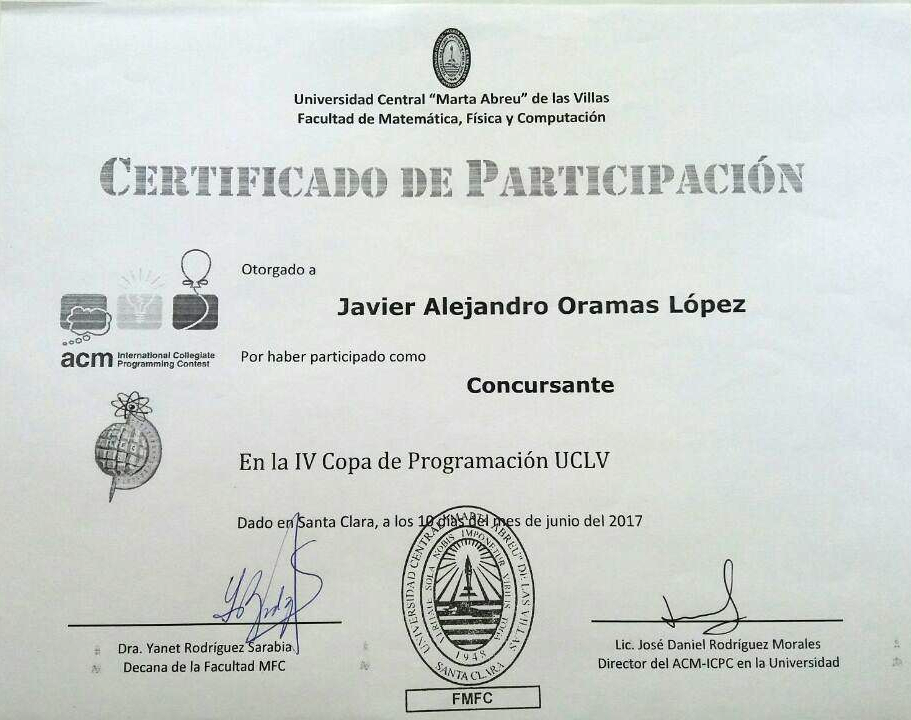
\includegraphics[width=\textwidth]{images/uclv_cup.png}
    \caption{Participation Certificate, IV Programming Cup, Universidad Central de Las Villas, screenshot 01/25/2022}
    \label{sec:uclv_cup}
\end{figure}


\begin{figure}[h]
    \centering
    
\includegraphics[width=\textwidth]{images/nac_contest.png}
    \caption{Certificate for Relevant Results obtained in the National Informatics Competition, Mach 2017, screenshot 01/25/2022}
    \label{sec:nac_contest}
\end{figure}


\begin{figure}[h]
    \centering
    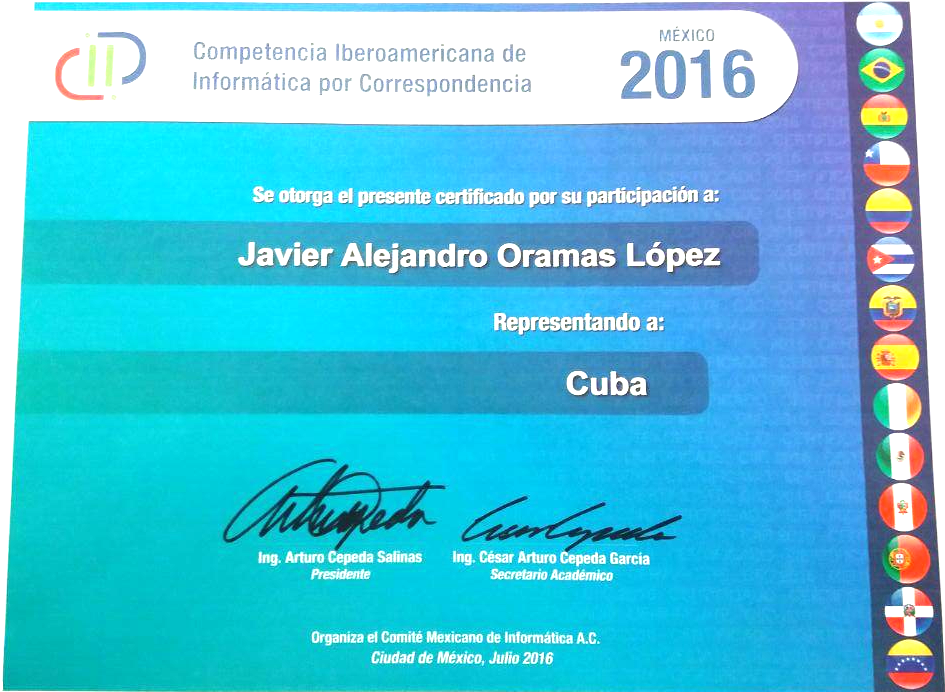
\includegraphics[width=\textwidth]{images/ibero.png}
    \caption{Certificate of Participation, Iberoamerican Computer Correspondence Competition, México 2016, screenshot 01/25/2022}
    \label{sec:ibero}
\end{figure}


\begin{figure}[h]
    \centering
    
\includegraphics[width=\textwidth]{images/preseleccion.png}
    \caption{Certificate from the Ministry of Education of Cuba for having integrated the National Preselection to the International Olympiads of Informatics. 2016, screenshot 01/25/2022}
    \label{sec:preseleccion}
\end{figure}


\begin{figure}[h]
    \centering
    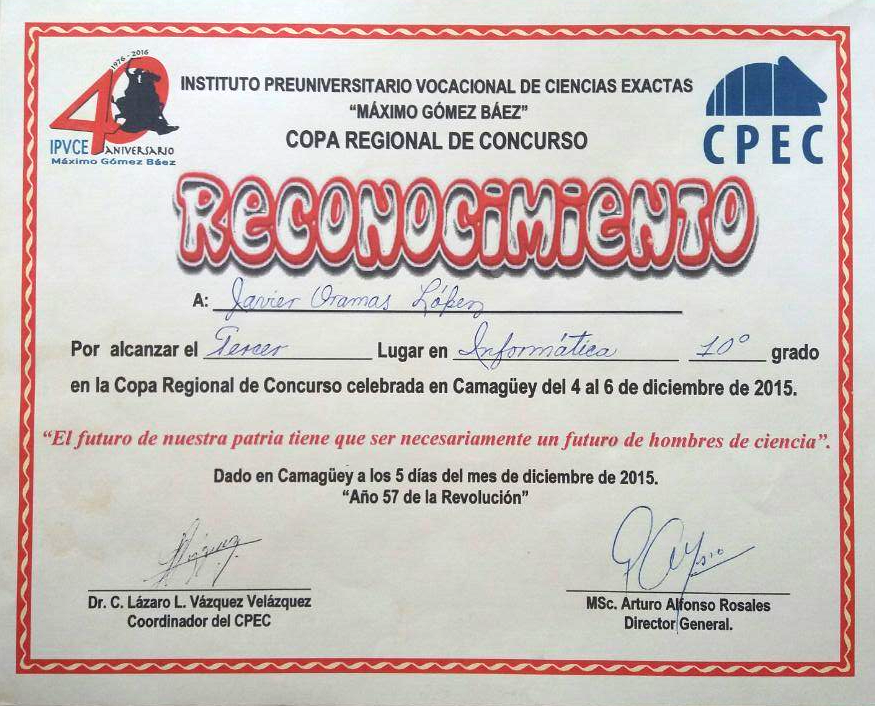
\includegraphics[width=\textwidth]{images/tinajon.png}
    \caption{Certificate for Third place obtained in the Regional Cup of Computer Science Competition, Camag\"uey December 2015, screenshot 01/25/2022}
    \label{sec:tinajon}
\end{figure}


\begin{figure}[h]
    \centering
    
\includegraphics[width=\textwidth]{images/2016nacional.png}
    \caption{Certificate of participation in the National Competition of the ACM-ICPC, Universidad Central de Las Villas, October 2015, screenshot 01/25/2022}
    \label{sec:nacional2016}
\end{figure}


\begin{figure}[h]
    \centering
    
\includegraphics[width=\textwidth]{images/2016local.png}
    \caption{Certificate of participation in the Local Competition of the ACM-ICPC, Universidad Central de Las Villas, September 2015, screenshot 01/25/2022}
    \label{sec:local2016}
\end{figure}

\begin{figure}[h]
    \centering
    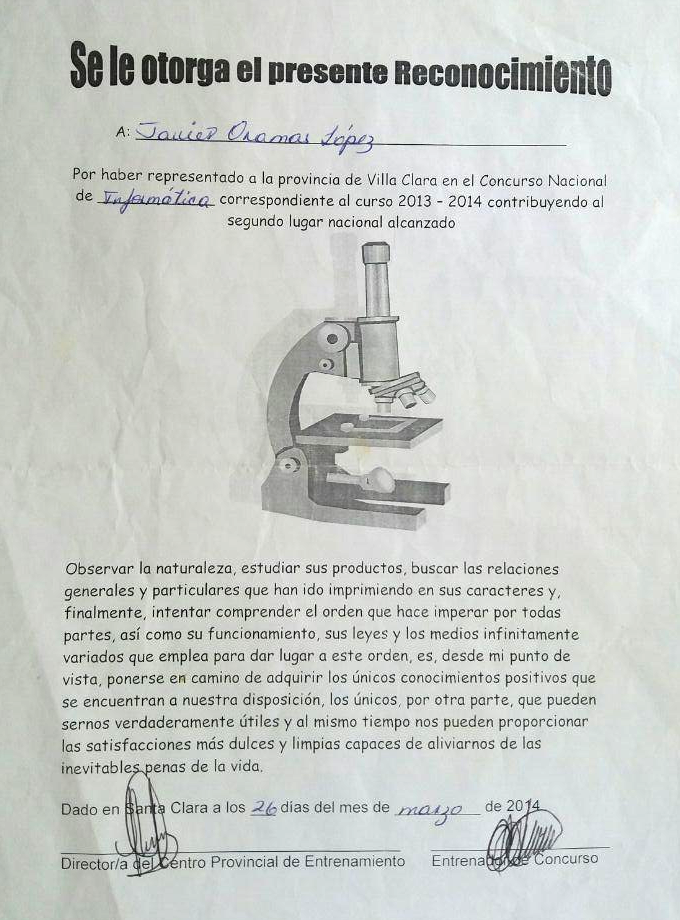
\includegraphics[width=\textwidth]{images/informatica.png}
    \caption{Recognition for second place obtained in the National Computer Science Competition, Marzo 2014, screenshot 01/25/2022}
    \label{sec:informatic}
\end{figure}

\end{document}
